% !TeX root = ../main.tex

\chapter{基于模型的优化}
\label{chap:optimization}
\section{流量预测}
\subsection{离散时间情况}
第\ref{chap:model}章中描述的模型建立在连续时间下。在实际的传输中考虑每个比特的情况会节省计算和存储的复杂度,因此
上述模型需要转换为离散情况。
在离散的情况下,式\ref{equ:time}中的$t_i$会按照当前的发送速率转换为每个比特上的ON或OFF状态。比如,延续时间长度为0.1ms的一帧在500kpbs的速率下,就对应50个比特的ON状态长度。

为了计算每一比特上对于ON/OFF状态的预测,最直观的方法是利用\emph{整数分解}进行预测。假设即将发送的帧长度为$L$比特,整数分解算法需要找到所有有序$k$元组$(l_1, \cdots, l_k)$,满足
\begin{equation}
	\sum_{i = 1}^{k} l_i = L,
\end{equation}
其中$k,l_i \in \mathbb{Z}^+,\,i = 1,\cdots,k$。每一个$l_i$都代表着当前ON/OFF状态持续的长度(以比特为单位)。在给定传输速率$r$的情况下,可以转换为实际长度时间$t_i = \frac{l_i}{r}$。依照经验分布函数,可以得到$l_i$出现的概率
\begin{equation}
p_{l_i} = 
\begin{cases}
f_{ON}^{-1}(t_i), \,i\, mod 2 = 1;\\
f_{OFF}^{-1}(t_i), \,i\, mod 2 = 0
\end{cases}
\end{equation}
那么,对于当前的$k$元组$(l_1, \cdots, l_k)$,其出现的概率为$\prod_{i}p_i$。对所有可能的分解依照其对应的出现概率进行加权,可以实现对每个比特发送时处于ON状态概率的预测。

但这种方法的复杂度很高,在第\ref{chap:evaluation}章有具体的评估数据。更适合该模型的方法是利用\emph{蒙特卡罗方法}进行模拟。在单次模拟中,当ON/OFF状态在相互转化时,利用均匀分布和经验累积分布函数按下式进行随机采样得到$l_i$:
\begin{equation}
l_i = \inf_l\{F_{ON/OFF}(l) < u_i\},
\end{equation}
其中$U_i \sim U[0,1]$。在进行$N$次模拟后,计算每个比特位值遇到ON状态的频率作为最终的预测。这里记预测后的结果为$(p_1, \cdots, p_L)$,其中$p_i$表示第$i$比特是ON状态的概率。

图\ref{fig:heatmap_256_500_mall}-\subref{fig:heatmap_256_500_lab}展示了不同环境、速率和帧长的情况下,使用蒙特卡罗方法进行500000次模拟的预测结果。图中显示的是每一比特上会是ON状态的概率。总的来看,在实验室和商场中ON状态更容易出现,而家庭环境中几乎都是OFF状态。这与之前的分析是相符合的——在商场和实验室中用户使用网络更加频繁,因此标签要发送的数据更容易搭上环境中的流量。另一方面,更高的传输速率和更短的帧长会更容易遇见ON状态,直观来讲,符合这两个条件的帧可以在当前环境中的Wi-Fi流量消失之前尽快完成传输。
\begin{figure}[t]
	\begin{minipage}[b]{.32\linewidth}
		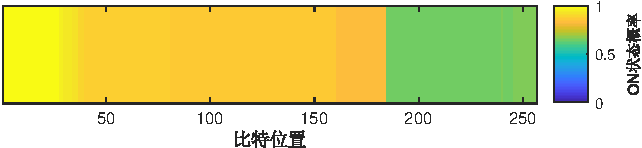
\includegraphics[width = \linewidth]{opt_figure1_256_500_mall-cropped}
		\subcaption{商场环境,256比特,500kbps。}\label{fig:heatmap_256_500_mall}
	\end{minipage}
	\hfill
	\begin{minipage}[b]{.32\linewidth}
		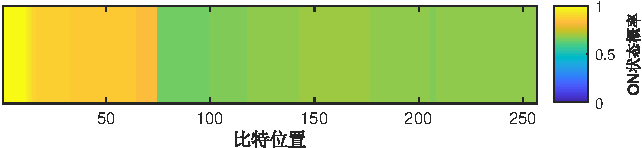
\includegraphics[width = \linewidth]{opt_figure1_256_200_mall-cropped}
		\subcaption{商场环境,256比特,200kbps。}\label{fig:heatmap_256_200_mall}
	\end{minipage}
	\hfill
	\begin{minipage}[b]{.32\linewidth}
		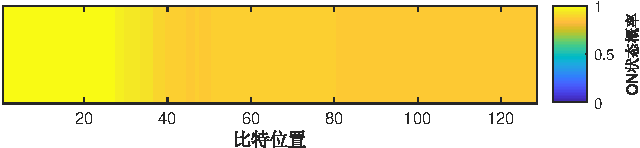
\includegraphics[width = \linewidth]{opt_figure1_128_500_mall-cropped}
		\subcaption{商场环境,128比特,500kbps。}\label{fig:heatmap_128_500_mall}
	\end{minipage}
	
	\begin{minipage}[b]{.32\linewidth}
		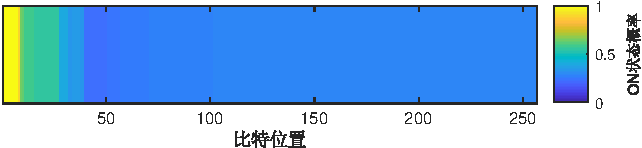
\includegraphics[width = \linewidth]{opt_figure1_256_500_home-cropped}
		\subcaption{家庭环境,256比特,500kbps。}\label{fig:heatmap_256_500_home}
	\end{minipage}
	\hfill
	\begin{minipage}[b]{.32\linewidth}
		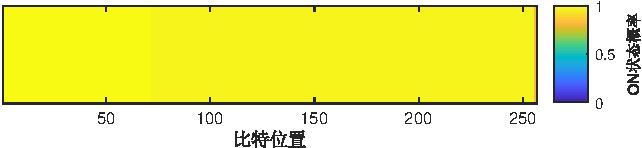
\includegraphics[width = \linewidth]{opt_figure1_256_500_lab-cropped}
		\subcaption{实验室环境,256比特,500kbps。}\label{fig:heatmap_256_500_lab}
	\end{minipage}
	\hfill
	\begin{minipage}[b]{.32\linewidth}
		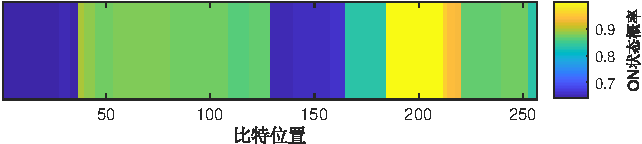
\includegraphics[width = \linewidth]{opt_figure2_256_500_lab_deperm-cropped}
		\subcaption{热力图(\subref{fig:heatmap_256_500_mall})置换后。}\label{fig:heatmap_perm}
	\end{minipage}
	\caption{不同环境、不同帧长、不同传输速率下的预测热力图。图中显示的是每一比特处于ON状态的概率。图(\subref{fig:heatmap_perm})展示了置换的效果。}\label{fig:heatmap}
\end{figure}

\subsection{预测对LDPC解码的影响}

LDPC的解码使用信念传播算法(Belief propagation)。对于传输的LDPC码字$x = (x_1, x_2, …, x_{L})$,记对应信道的输出为$y = (y_1, y_2, …, y_{L})$。LDPC解码算法的输入是每一比特的对数似然比(Log-likelihood ratio, LLR):
\begin{equation}
\label{equ:llr}
L(x_i)=\log\left(\frac{\Pr(x_i=0|y_i)}{\Pr(x_i=1|y_i)}\right)
\end{equation}
在算法在$L(x_i)$的基础上不断迭代,更新对每一个比特$x_i$的LLR估计。在算法中,传输信息的比特和负责校验的比特之间会相互交换LLR信息,这也是算法名称的由来。在算法中,一个重要的假设是校验节点与信息节点之间传递的信息是相互独立的,因此越长的最小循环长度越满足此假设,从而解码效果更好。

值得注意的是,初始LLR的计算是需要对信道的先验的。如果简单的考虑为加性高斯信道,会导致LDPC解码的效果很差;而结合对信道的先验的情况下,式\ref{equ:llr}可以写为:
\begin{equation}
\label{equ:llr_new}
L(c_i)=\log\left(\frac{ p_i \frac{1}{1+\rho_i} + \frac{1}{2} (1-p_i) }{ p_i \frac{1}{1+1/\rho_i} + \frac{1}{2} (1-p_i)  }\right),
\end{equation}
其中$\rho_i = \Pr\{y_i|x_i=1\}/\Pr\{y_i|x_i=0\}$。
\section{依据预测优化}

\subsection{置换}
\label{subsec:perm}
在针对每一比特的预测概率基础上,可以引入交织(置换)机制使得帧可以以更高的概率应对突发错误,以提高系统的可靠性。对于长度为$L$比特的帧$F$,假设当前使用的是$(n,k)$的码,
%\footnote{如果使用里德-所罗门码也是相似的,将长度$L$换为$L/8$即可}。
通常情况下,$L$都是可以被$n$整除的,不足的部分也可以通过填充实现。假设$L = bn$,那么在编码过程中会对原始数据分成$b$块。由于我们已知每一比特遇到OFF状态的概率,可以通过\emph{将高概率出现OFF状态的位置均匀置换到每一块中}。我们的目标是寻找一个置换$\sigma^\ast$,使得
\begin{equation}
\label{equ:sigma}
\sigma^\ast = \argmax_\sigma \Var \{ (z_1, \cdots, z_b) \} 
\end{equation}
其中$z_i, i = 1,\cdots,b$是置换后的帧$sigma(F)$每$i$块中可能出现OFF的个数。考虑到R-S码适合处理连续的错误,式\ref{equ:sigma}还需要服从连续性条件,
即\emph{处于OFF状态的比特之间要尽量处于相邻的位置}。由于预测给出的是概率值,因此我们会设置一个阈值,概率小于阈值的会被认定为OFF。图\ref{fig:heatmap_perm}展示了对图\ref{fig:heatmap_256_500_mall}进行置换后的热力图,集中在第二块中的易遇见错误的比特会被均匀分散到两块中,从而提升可靠性。

\subsection{动态参数调节}

在采用不同的帧长和传输率的情况下,即便是基于相同的累积分布函数,也会产生不同的预测效果。直观来讲,编码能够回复的范围内尽量提升码率可以让通信更高效。
%一般来说,在帧长一定的情况下,选择越高的传输率由越高的机会在ON状态下发送完数据;在传输率一定的情况下,选择越长的帧长会有更高的可能性再发送的过程中遇见OFF状态,但是会有更高的吞吐量。同样,对环境的预测也会影响码率的选择:如果预测环境中Wi-Fi流量比较繁忙,那么可以提升码率,以达到更高的吞吐量;如果预测环境中会出现较多的OFF状态,会选择降低码率,已保证该帧可以正确传输。
假设当前使用的编码在每一块中可以纠正$t$比特错误,在最理想的情况下,结合置换一共可以纠正$bt$比特的错误。将最有可能出现OFF状态的$bt$比特利用码进行纠正,剩下所有比特位置全部为ON状态的概率可以由下式计算:
\begin{equation}
p_{success} = \frac{\prod_{i = bt+1}^{L} p_i^{'}}{n^\alpha},
\end{equation}
其中$p_i^{'}$是对原有预测$p_i$升序排列后的概率,分母用来平衡长度影响的参数,因为预测越长越易出现错误预测。在实际的计算中采用$\alpha=2.5$。进一步,在给定帧长、传输率和码率的选择范围下,我们求解下式的最优化问题:
\begin{equation}
\label{equ:dynamic_parameter}
L^\ast, r_{data}^\ast, r_{code}^\ast = \argmax_{L, r_{data}, r_{code}} \frac{r_{data}}{L}\cdot L\cdot r_{code} \cdot p_{success},
\end{equation}
其中$L,r_{data},r_{code}$依次指帧长、传输率和码率。本质上,式\ref{equ:dynamic_parameter}是在求解单位时间内可以正确传输的比特数。由于$p_{success}$一般会很小,因此采用对数形式的式\ref{equ:dynamic_parameter}。